\hyphenation{se-para-tion}
\hyphenation{theo-re-ti-cal}
\hyphenation{handed-ness}
\hyphenation{fo-llo-wing}
\hyphenation{ac-cor-ding}

%______________________ Theory ______________________
\chapter{Theory}
\label{ch:theory}

In the previous chapter we introduced the SM and discussed particles and interactions that the SM as a theory describes. In this chapter we will discuss first the general mathematical formalism of the SM and in the second part we will focus on the double Higgs theory in the BSM	.

SM is the only accepted mathematical theory that has been extremely successful describing the interactions of elementary particles and fields. SM includes all known interactions except gravity. 

%______________________ INTRODUCCION ______________________
\section{Lagrangian formalism of the Standard Model}


The SM uses the Lagrangian mechanics as the mathematical approach to describe quantitatively the interactions of elementary particles and fields. 
The SM Lagrangian can be split into four main contributions \cite{Mozer:2016wzi}:
\begin{equation}\label{lagr_SM}
\Lagr_{SM} = \Lagr_{YM} + \Lagr_{ferm} + \Lagr_{H} + \Lagr_{Yuk} 
\end{equation}

This equation contains the following terms:

\begin{itemize}
\item gause bosons and their interactions, $\Lagr_{YM} $
\item fermions and their interactions with the gauge bosons, $\Lagr_{ferm}$
\item Higgs boson, its self-interaction, and interaction with the gauge bosons to give them mass, $\Lagr_{H}$%, which is not possible solely by the $\Lagr_{YM}$
\item fermions and their interactions with the Higgs boson, which through the Yukawa mechanism give mass to fermions $\Lagr_{Yuk} $
\end{itemize}
 


The first term in the SM Lagrangian in full can be written as:
\beqn\label{lagr_YM}
\Lagr_{YM} = 	-\frac{1}{4}W^i_{\mu\nu}(x)W_i^{\mu\nu}(x) -\frac{1}{4}B_{\mu\nu}(x)B^{\mu\nu}(x) -\frac{1}{4}G^a_{\mu\nu}(x)G_a^{\mu\nu}(x)
\eeqn

where

\begin{align}
B_{\mu\nu}(x)   \equiv & \partial_\mu B_\nu -  \partial_\nu B_\mu \label{B_tensor} \\ 
W^i_{\mu\nu}(x) \equiv & \partial_\mu W^i_\nu(x) - \partial_\nu W^i_\mu(x) - g\varepsilon^{ijk}W^j_\mu W^k_\nu \label{W_tensor}\\
G^a_{\mu\nu}(x) \equiv & \partial_\mu G^a_\nu(x) - \partial_\nu G^a_\mu(x) - g_s f^{abc}G^b_\mu G^c_\nu \label{G_tensor}
\end{align}

\noindent with indexes $i,j,k = 1,2,3$ and $a,b,c = 1, ..., 8$. According to the Noether's theorem, each symmetry is intrinsically connected to the conservation law \cite{Sardanashvily:2143630}. The fields in the $\Lagr_{YM} $ are connected to their corresponding underlying symmetries. For instance, $B_{\mu\nu}$ corresponds to $U(1)$ symmetry of the weak hypercharge $Y_k$, $W^i_{\mu\nu}$ corresponds to $SU(2)_I$ symmetry of the weak isospin $I^i_{w}$, and $G^a_{\mu\nu}$ corresponds to $SU(3)_c$ symmetry of the QCD color charge. The "B" field is a kinematic term, "W" and "G" terms describe interactions among the bosons, $g$ and $\varepsilon$ are $SU(2)$ coupling and structure constants, finally $g_s$ and $f$ are coupling and structure constants for $SU(3)$.

The second term in the SM Lagrangian shows how fermions interact with the gauge bosons. Notice, that the mass terms are still absent:
\beqn\label{lagr_ferm}
\Lagr_{ferm}= i \bar{\Psi}_L \slashed{D} \Psi_L  + i \bar{\psi}_{l_{R}}  \slashed{D} \psi_{l_{R}} +
i \bar{\Psi}_Q \slashed{D} \Psi_Q  + i \bar{\psi}_{u_{R}}  \slashed{D} \psi_{u_{R}} +
 i \bar{\psi}_{d_{R}}  \slashed{D} \psi_{d_{R}}
\eeqn

Above $\Psi$ represents a doublet of a charged lepton and a corresponding neutral lepton within the same lepton family of $SU(2)_L$, the letter Q is reserved for a family of quarks, and $\psi_R$ describes a right-handed leptonic singlet.

Gauge boson interactions are present due to the derivative term:
\begin{align}\label{cov_der2}
D_\mu = \partial_\mu + ig I_w^i W_\mu^i+ ig' Y_w B_\mu + ig_s T_c^a G_\mu^a\\ 
\end{align}

Physical fields in this notation are represented by a linear combination of W and B fields:
\begin{align}\label{neutral_fields}
A_\mu = &  B_\mu \cos\theta_W + W^3_\mu \sin\theta_W \\ 
Z_\mu = & -B_\mu \sin\theta_W + W^3_\mu \cos\theta_W \nonumber 
\end{align}
\noindent where $\theta_W$ is known as the \ti{Weinberg angle} \cite{Weinberg:799984}.

With the first two terms of the SM Lagrangian we obtain a valid theory of fermions and bosons, however, these particles are massless in this theory \cite{Wolf:2015kua}, which evidently contradicts the reality. To solve this issue and to ensure that weak bosons are massive, we need to introduce a Higgs field. Higgs mechanism enters the SM Lagrangian through the corresponding Higgs Lagrangian term given by 
\beqn\label{lagr_higgs}
\Lagr_H=(D_\mu\Phi)^\dagger(D^\mu\Phi) - V(\Phi) , \qquad V(\Phi)= - \mu^2(\Phi^\dagger\Phi) + \frac{\lambda}{4}(\Phi^\dagger\Phi)^2
\eeqn

\noindent where

\beqn
\Phi = \binom{\phi^+}{\phi^0 = (v+H + i\chi)/ \sqrt{2}} \quad \text{with} \quad v = 2 \sqrt{\frac{\mu^2}{\lambda}}
\eeqn

Here $\mu$ and $\lambda$ are parameters of the Higgs potential. The Higgs boson mass is proportional to the $\mu$ parameter. In 2012 with precise single Higgs boson mass measurements from both ATLAS and CMS experiments we determined the value of $\mu$. Since that time many analyses at CERN have been targeting the measurement of the $\lambda$ parameter, because it is related to the shape of Higgs potential. The simplest interaction that is probing the Higgs potential directly is the Higgs boson self-coupling. One of such processes is the non-resonant double Higgs boson production. With double Higgs boson physics being such a valuable tool to determine the  

After the SSB, the value of the Higgs field vacuum expectation value $v$ shown above can be expressed in terms of $\mu$ and $\lambda$ \cite{MonroyMontanez:2639240}. See Fig. \ref{hp2d} for an illustration for the Higgs potential before and after SSB.

\begin{figure}[H]
\centering
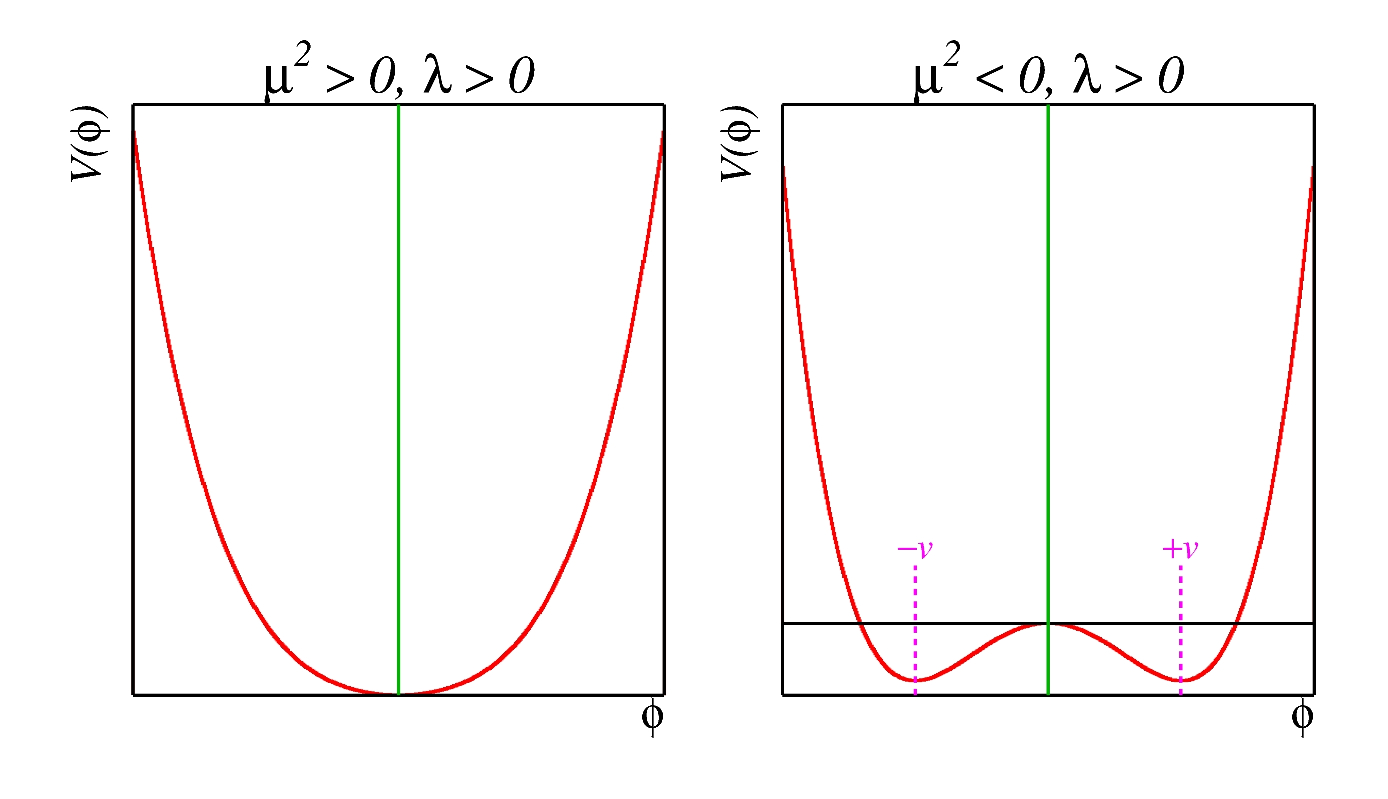
\includegraphics[width=0.6\textwidth]{hp2d}
\caption[SSB Potential form]{Shape of the Higgs potential before and after SSB that is determined at the leading orders by $\mu$ and $\lambda$ parameters. }
\label{hp2d}
\end{figure}

After adding $\Lagr_H$ and rearranging terms, bosons have masses given by:

\beqn
M_W = \frac{gv}{2}, \quad  M_Z = \frac{M_W}{\cos{\theta_W}}, \quad M_H = \sqrt{2\mu^2}
\eeqn
 
The final contribution to the SM Lagrangian is the Yukawa term, and Yukawa Lagrangian is given by:
\beqn\label{lagr_Yuk}
\Lagr_{Yuk}=  - i \bar{\Psi}_{L}  G_l  \psi_{l_{R}} \Phi
- i \bar{\Psi}_{Q}  G_u  \psi_{u_{R}} \tilde{\Phi}
- i \bar{\Psi}_{Q}  G_d \psi_{d_{R}} \Phi + h.c.
\eeqn

where $\tilde{\Phi} = i \sigma^2 \Phi^*$

The masses of fermions enter the equations through the $3 \times 3$ matrices G, which are not known from the theory and are the parameters of the SM. The mass of each fermion is proportional to the Yukawa coupling of the corresponding fermion to the Higgs boson, see Fig. \ref{coupling_ff}.

\section{Beyond the Standard Model}

Several BSM theories \cite{Huang:2017nnw, Dolan:2012ac, Kanemura:2016tan} predict a resonant production of the double Higgs boson events through a heavy narrow width ($\sim O(1-10)$ GeV) resonance, which could be spin 0 or spin 2 particle \cite{Sirunyan:2018iwt}. In this particular analysis data is compared with respect to predictions from the Warped Extra Dimensions theory (WED) \cite{Oliveira:2014kla}. WED theory to address the hierarchy problem adds additional fifth dimension to the 4-dimensional (4D) space-time. In the framework that Randall and Sundrum (RS) \cite{Randall:1999ee} followed, 4D space is nothing but an EFT approximation of the higher dimensional space, where the radion or graviton may exist as Kaluza-Klein (KK) \cite{Uzawa:1999pg} excitation modes at the TeV scale. Since LHC had provided us with no evidence of the SM particles interacting with the additional RS dimensions, it is postulated that they are confined to 3-brane, or a so-called wall. At the same time, gravity, which is not in the SM, can propagate freely in the full higher-dimensional space, so-called bulk. If/when the bulk is compactified, it may produce KK modes of the gravitons. In this analysis RS model with parameter k of the order of Planck scale and $\bar{M}_{Pl}$, a reduced 4D $M_{Pl}$ which is a function of the 5D Planck scale M and a parameter k with $k<M$, are assumed to satisfy the constraint $0.01 \leq k / \bar{M}_{Pl} \leq 1$, because values outside of this range are not applicable/or overcomplicate the theory \cite{Davoudiasl:1999jd}. Considered in this measurement graviton and radion are thus RS KK graviton and RS radion particles that emerge in RS scenario with the excitation or a KK state mass of the order of TeV. 

If we denote a part of the KK 5D wave function, often called a profile, as $f^{(n)}_X(\phi)$, where n is referred to the KK$^{th}$ mode, then the graviton 4D profile wave-function can be expressed as $h^{(n)}_{\mu\nu}(x_\mu)(f^{(n)}_X(\phi))$ and the zero-th mode of this function would correspond to the graviton that is a gravity mediator. Its effective mass is of the order of TeV. The Lagrangian describing the interaction of the graviton with the SM fields is given then by 

\beqn\label{lagr_graviton}
\Lagr_{graviton}=  - \frac{x_1\tilde{k}}{m_G} h^{\mu\nu(1)} \times d_i T^{(i)}_{\mu\nu},  
\eeqn
where $T^{(i)}_{\mu\nu}$ is a 4D canonical energy-momentum tensor \cite{Forger:2003ut} for the SM field $i$ and $d_i$ is an integral of the profiles of the SM fields and KK gravitons. $\tilde{k}$ is a free parameter inversely proportional to the Planck mass and varies from 0.01 to 1 when $M_{graviton}$ is from 100 to 1500 GeV. 

For radion the Lagrandian is similar and is given by:
\beqn\label{lagr_radion}
\Lagr_{radion}=  - \frac{r}{\Lambda_R} \times a_i T^{\mu (i)}_{\mu},  
\eeqn
where $\Lambda_R$ is a scale parameter proportional to the Planck mass and $r$ is a 5D Radion field. If we make an assumption that the profiles of the graviton and radion are localised at the TeV scale, then the coupling of them to the massive SM fields is of the order of 1. Throughout this thesis, theory curves contain model results for the case $\tilde{k}=0.1$ and $\Lambda_R = 3 $ TeV.  

In this analysis the gravitons/radions in the search are expected to be produced by a gluon fusion mechanism. Five Feynman diagrams describe this process, two of which are present in the SM (a "box" and a "triangular" diagrams on Fig. \ref{SM_HH}), and the other three are a BSM extension of the SM (BSM contact interaction diagrams on Fig. \ref{BSM_HH}).   



\begin{figure}[H]
  \centering
    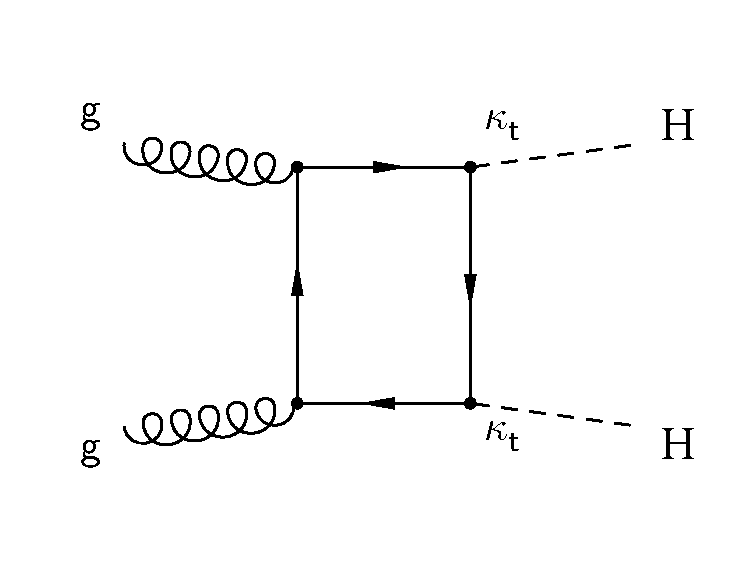
\includegraphics[width=0.49\textwidth]{hh_nonresonant_eft_02}
     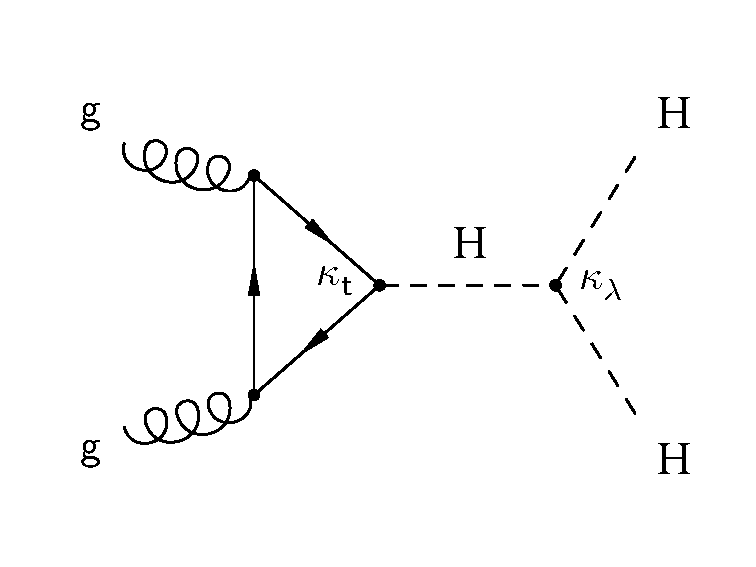
\includegraphics[width=0.49\textwidth]{hh_nonresonant_eft_01}
    \caption{SM double Higgs boson production.}
    \label{SM_HH}
\end{figure}

In the SM two main diagrams interfere destructively and the total cross section is thus lowered (Fig. \ref{hh_comparison} on the right). The box diagrams dominates the double Higgs boson production and peaks near 400 GeV. An extensive study has been performed by theorist for the future 100 TeV collider \cite{Chen:2014xra,}. However, since the kinematic distribution of the double Higgs mass remains to a high degree unchanged  between 13 and 100 TeV (see Fig. \ref{hh_comparison} on the left), we can extrapolate 100 TeV results to to those available at the current LHC machine energy. Fig. \ref{hh_comparison} has "nl" term, which denotes the contribution from the new non-linear $t\bar{t}HH$ interaction if this new coupling exists \cite{Contino:2012xk}. 


\begin{figure}[H]
  \centering 
    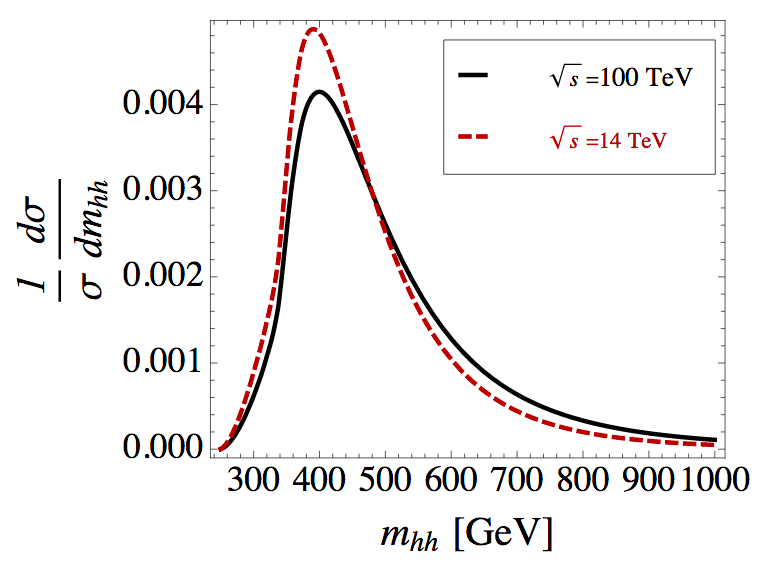
\includegraphics[width=0.49\textwidth]{hh_14_100_comparison}
    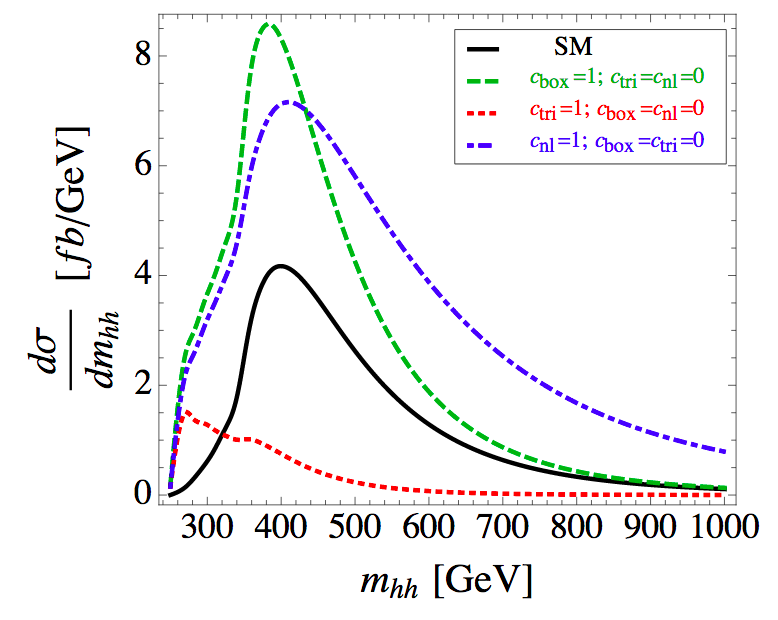
\includegraphics[width=0.49\textwidth]{hh_sm_comparison}
    \caption{Left: comparison of the double Higgs boson mass distribution at the LO at 14 and 100 TeV center-of-mass energy, Right: the total SM HH cross section and the box and the triangular contributions ("box" and "tri" at the plots).}
    \label{hh_comparison}
\end{figure}


It is also interesting to measure BSM contact interaction couplings and a future non-resonant version of this analysis will target that. In this case, $c_2$, the coupling of two heavy quarks with two Higgs bosons, $c_{2g}$, the coupling of two gluons with two Higgs bosons, and $c_g$, the direct coupling of the gluons to the Higgs boson will be studied (see Fig. \ref{BSM_HH}). 

\begin{figure}[H]
  \centering
    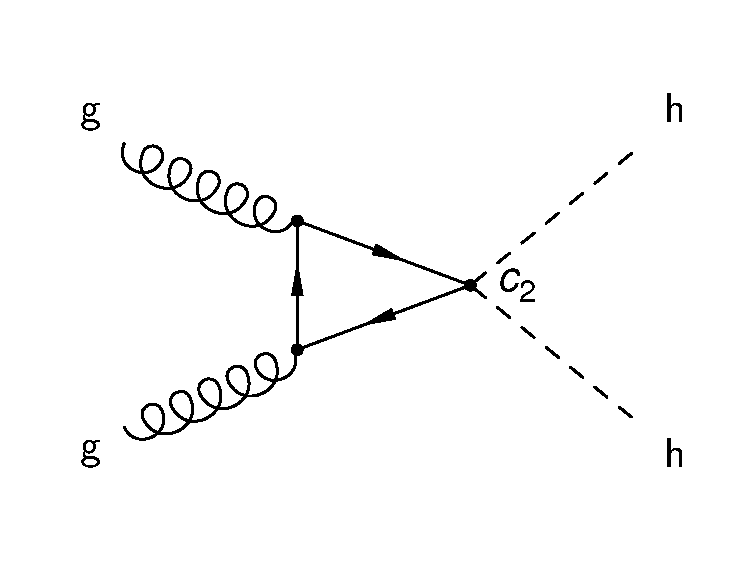
\includegraphics[width=0.49\textwidth]{hh_nonresonant_eft_03}
    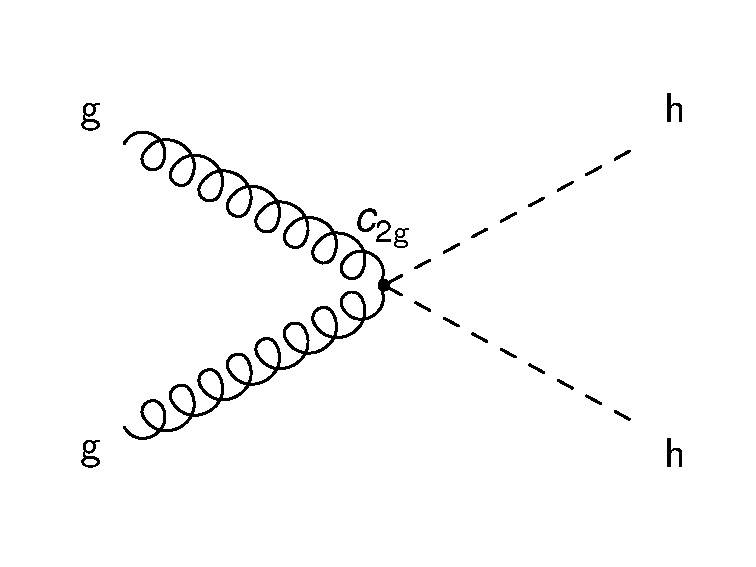
\includegraphics[width=0.49\textwidth]{hh_nonresonant_eft_04}\\
     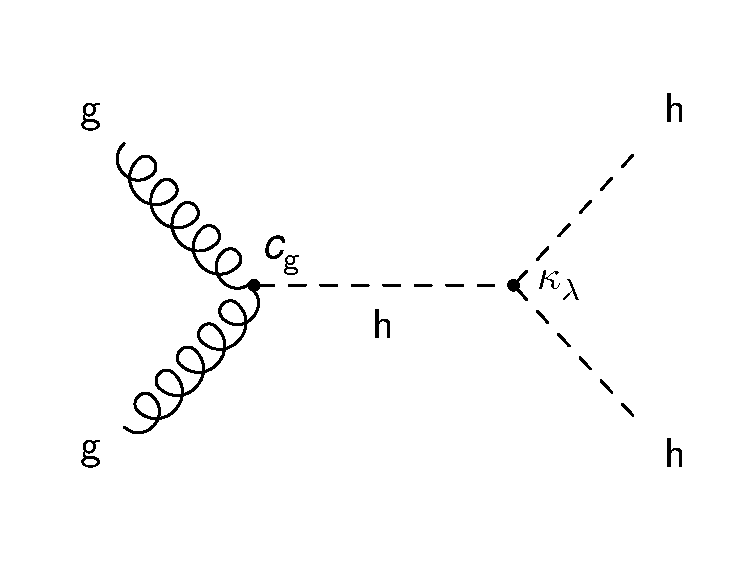
\includegraphics[width=0.49\textwidth]{hh_nonresonant_eft_05}
    \caption{BSM double Higgs boson production.}
    \label{BSM_HH}
\end{figure}


Now it is time to discuss the decay of the double Higgs system. 
This analysis considers separately graviton and radion decays into two SM Higgs bosons with the subsequent decays of one Higgs boson to a pair of b quarks, and the other Higgs boson to W or Z boson pairs. W bosons are allowed to decay only leptonically. For Z boson decays, the signature is characterised by the on-shell Z boson decaying into a lepton pair and the off-shell Z boson decaying to invisible (neutrinos)(see Fig. \ref{HH_signature}). 

\begin{figure}[H]
  \centering
    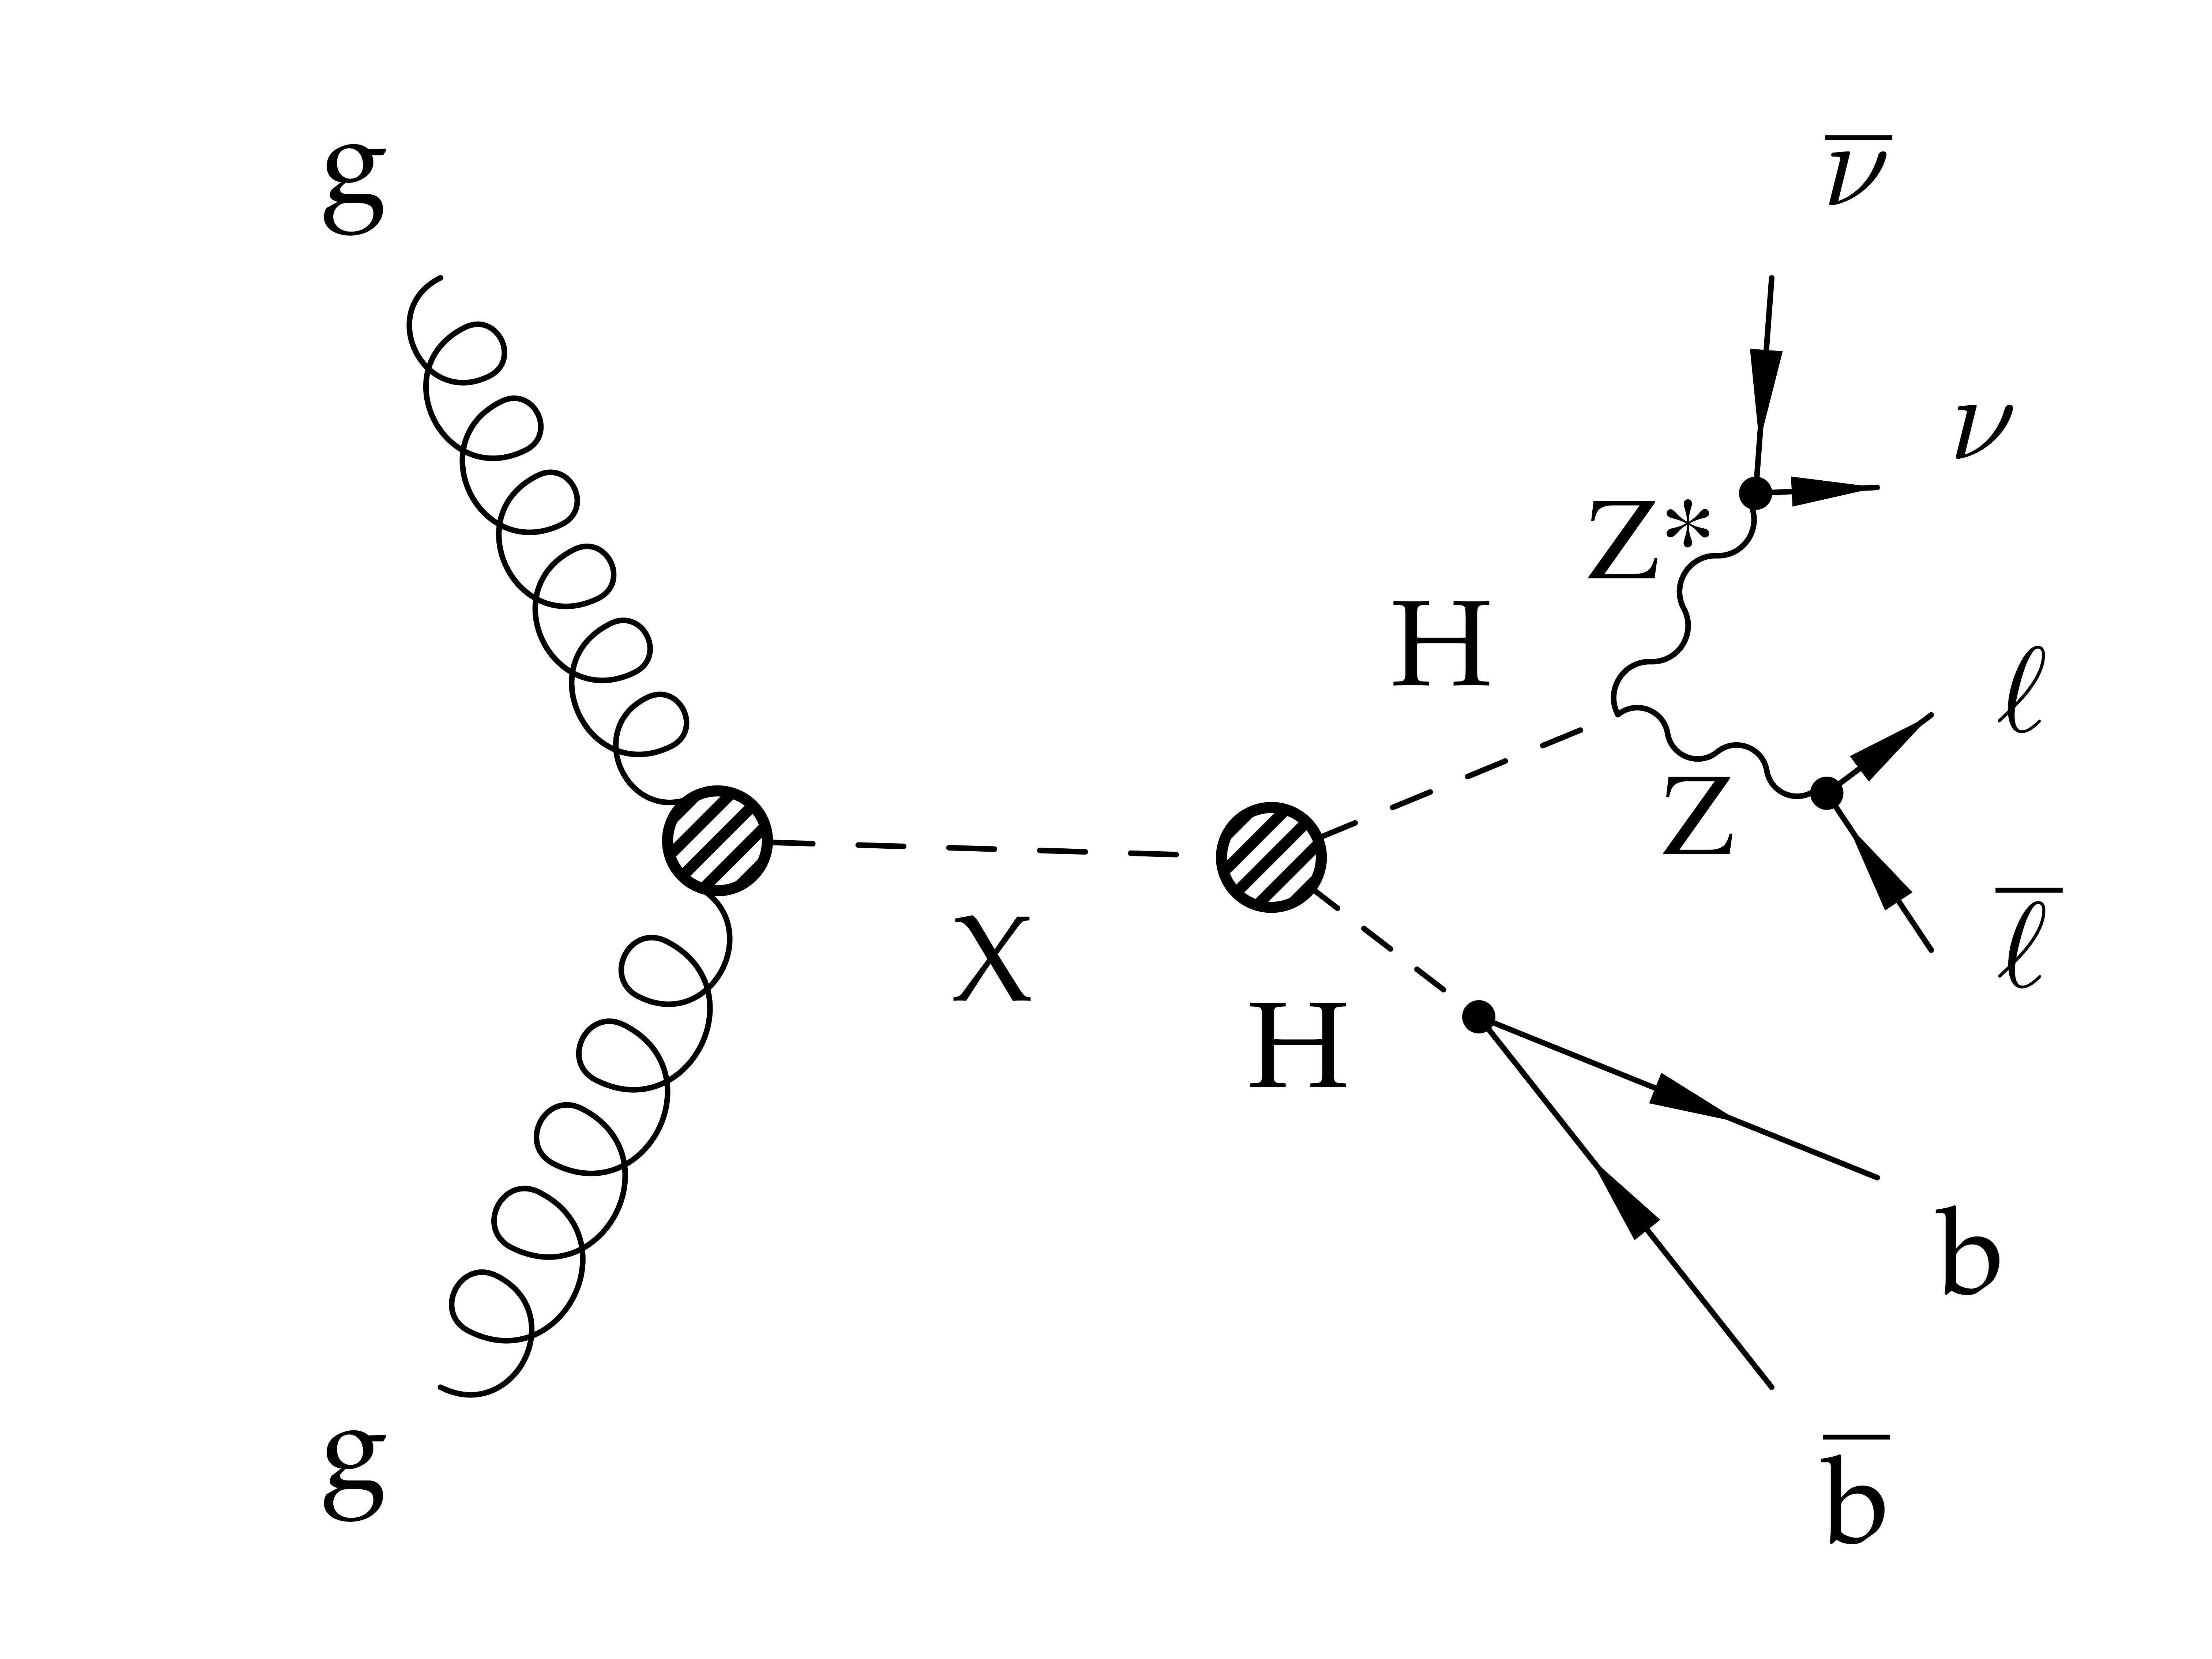
\includegraphics[width=0.50\textwidth]{HH_signature.png}
    \caption{Double Higgs decay in the 2 b, 2 lepton, and 2 neutrino final state. }
    \label{HH_signature}
\end{figure}

Before we finish this chapter, it is instructive to show all the decay channels of the double Higgs system to the SM particles, which is summarised in the Fig. \ref{BR}. This thesis explores the branching fraction of the double Higgs boson decay through $bbZZ$ in the two b quarks, two leptons, and two neutrinos final state, which equals approximately $2.8 \%$. 

\begin{figure}[H]
  \centering
    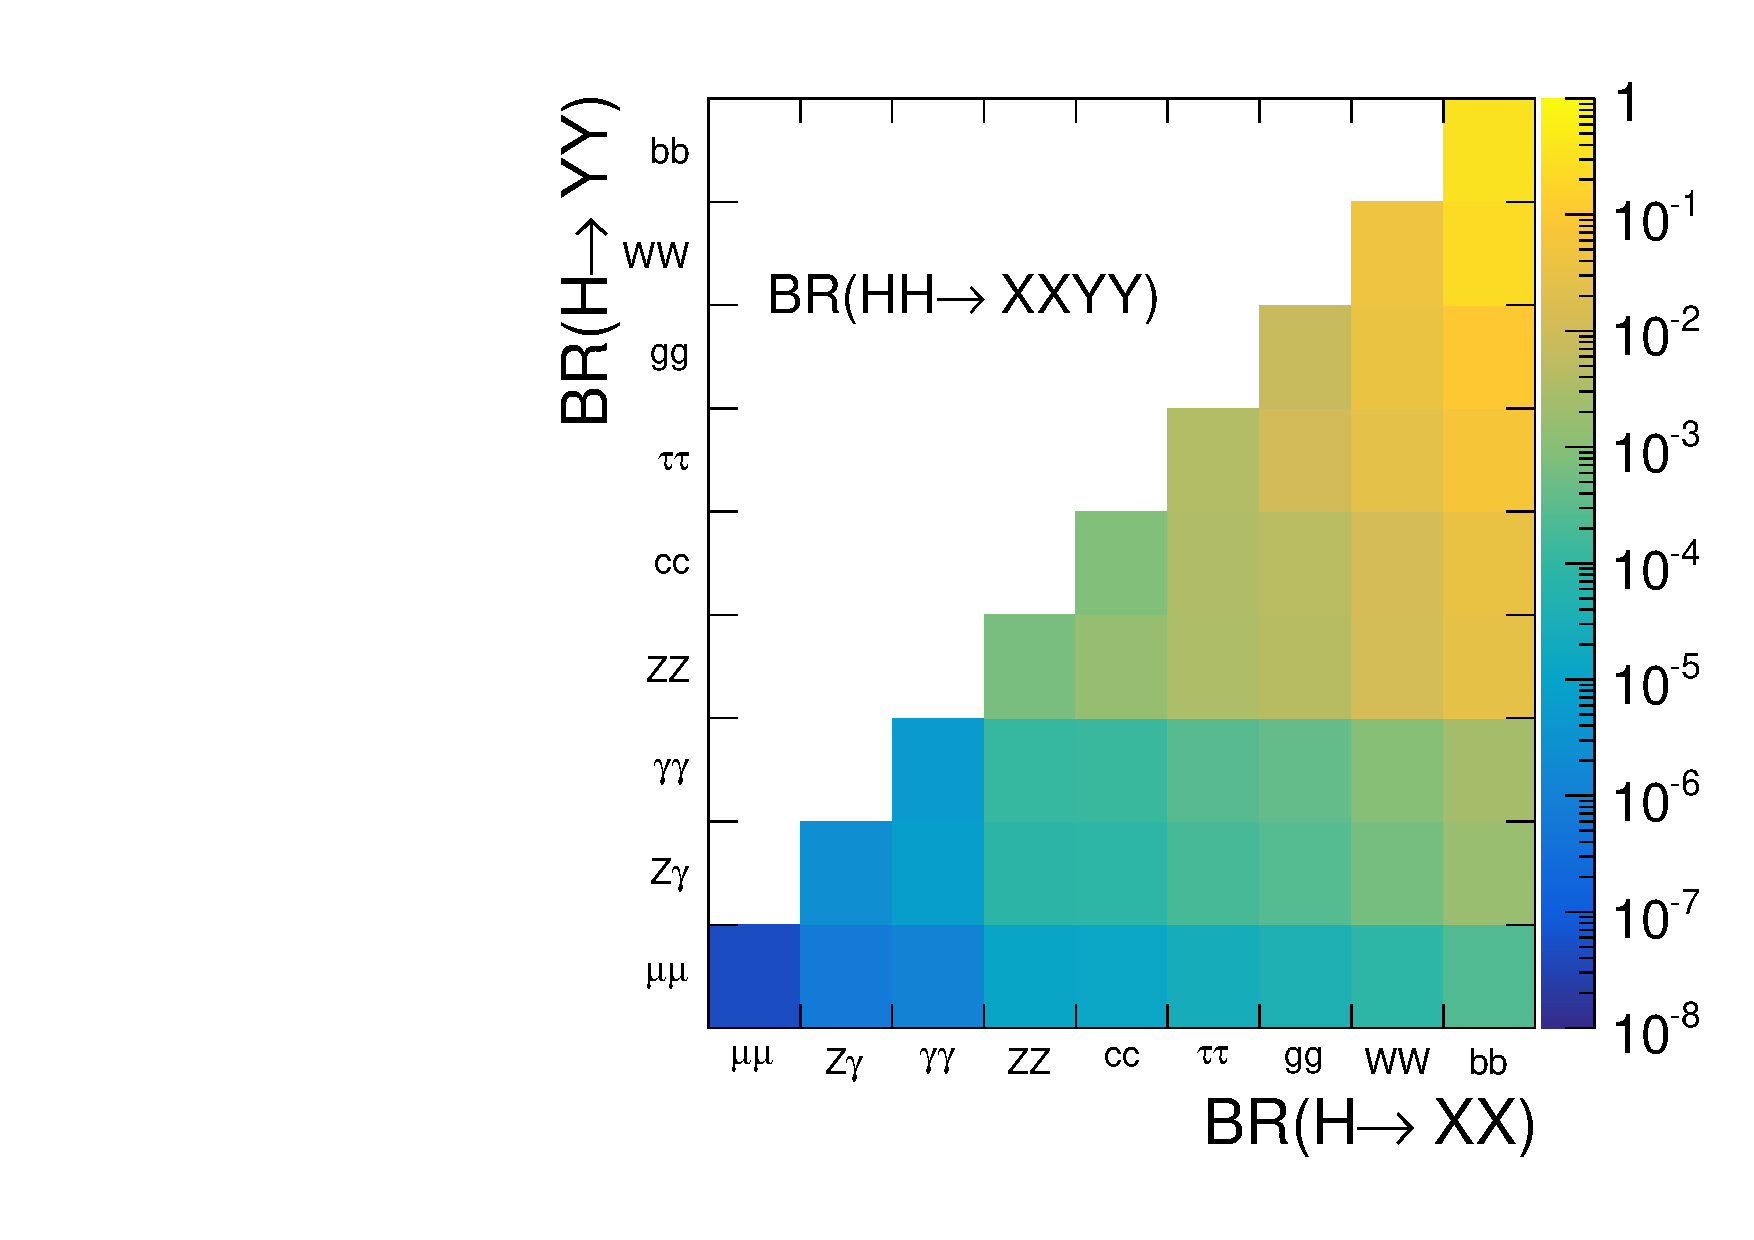
\includegraphics[width=0.50\textwidth]{BR}
    \caption{Double Higgs decay channels according to the SM branching fractions.}
    \label{BR}
\end{figure}



